\documentclass[8pt]{beamer}

\setbeamertemplate{background canvas}[vertical shading][bottom=cyan!10,top=blue!10]

\usetheme{Warsaw}
\usefonttheme[onlysmall]{structurebold}

% pour le fichiers .pdf
\usepackage{graphicx}
\usepackage{color}
% pour les fichiers .png
% \usepackage{pgf,pgfarrows}
% \usepackage{pgf,pgfarrows}
\usepackage{amsmath,amssymb}
\usepackage[latin1]{inputenc}
\usepackage[T1]{fontenc}
%\usepackage[french]{babel}
\usepackage{textcomp}
\usepackage{Math_Notations}
\usepackage{multitoc}
\usepackage{mdwtab}
\setbeamercovered{dynamic}
\DeclareMathOperator*{\argmin}{argmin}

\title[OpenTURNS Developer training]{OpenTURNS Developer training\\Elements of architecture}
\author[OpenTURNS Consortium, 2019]
{
  Trainer : R�gis LEBRUN \\
  EADS/IW/SE/AM \\
  regis.lebrun@eads.net
}



\date[March 22-25th 2011]
{
  Developers training \\

  \begin{center}
    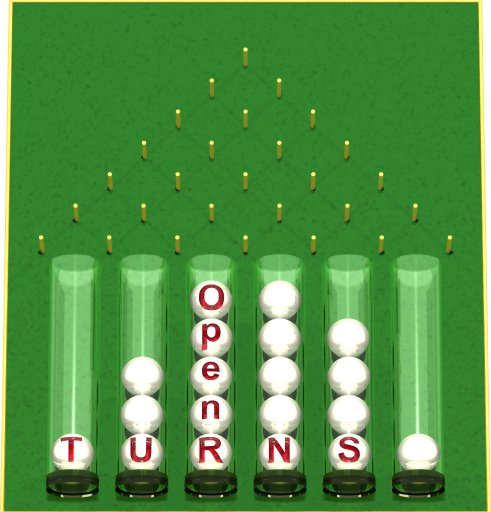
\includegraphics[height=2cm]{logoOT.jpg}
  \end{center}
}

\subject{OpenTURNS Developers Training}

% \part<presentation>{Corps de presentation}


\begin{document}

\frame{\titlepage}

% necessaire pour la table des matieres
\part{Main part}

% table des matieres
\begin{frame}
  \Large
  \frametitle{Elements of architecture}
  \tableofcontents[part=1]
\end{frame}
\section[]{Introduction}
\begin{frame}
  \frametitle{Introduction}
  \begin{block}{Objectives}
    The objectives of this course are:
    \begin{itemize}
    \item To present the main programing paradigms used in OpenTURNS;
    \item To present some of the most used design patterns;
    \item To illustrate these points based on a specific hierarchy: the distribution hierarchy.
    \end{itemize}
  \end{block}
\end{frame}
%%%%%%%%%%%%%%%%%%%%%%%%% 
% The OpenTURNS package %
%%%%%%%%%%%%%%%%%%%%%%%%% 
\section[Main architectural choices]{Main architectural choices}
%%%%%%%%%%%%%%%%%% 
% Global picture %
%%%%%%%%%%%%%%%%%% 
\begin{frame}
  \frametitle{A few words about C++}
  \begin{block}{Why C++?}
    \begin{itemize}
    \item \alert{The C++ language is by many aspects an awful language}, so there is no point to start a programing language war with a C++ developer: he already knows all that you can say!
    \item Nobody can pretend to be a C++ expert, even its conceptors, even the compiler developers! As such, it is always possible to blame gcc for a bug of your own...
    \item Despite its numerous defects (not really an object language, too low level for the object community, too high level for the performance-inclined developers), it allows for the definition of a \alert{domain specific language} that hide most of the ugly aspects from the numerician in favor to a much natural language where the concepts are named in the proper way, with the attended behaviour.
    \item It was one of the key points that lead to the choice of C++ as a programming language for OpenTURNS: the separation between the architect in charge of the low-level aspects of the progamming language, and the numerician in charge of the algorithmic development.
    \end{itemize}
  \end{block}
\end{frame}
%%%%%%%%%%%%%%%%%% 
% Global picture %
%%%%%%%%%%%%%%%%%% 
\begin{frame}
  \frametitle{Resource management}
  \begin{block}{Resource Acquisition Is Initialization (RAII) paradigm}
    Definition [From wikipedia]: \alert{Resource Acquisition Is Initialization} is a \alert{programming idiom} used in several object-oriented languages like C++, D and Ada. The technique was invented by Bjarne Stroustrup[1] \alert{to deal with resource deallocation in C++}. In this language, the only code that can be guaranteed to be executed after an exception is thrown are the destructors of objects residing on the stack. \alert{Resources} therefore \alert{need to be tied to the lifespan of suitable objects in order to gain automatic reclamation}. They are \alert{acquired during initialization}, when there is no chance of them being used before they are available, and \alert{released with the destruction} of the same objects, which is guaranteed to take place even in case of errors.\\

    \alert{RAII is vital in writing exception-safe C++ code}: to release resources before permitting exceptions to propagate (in order to avoid resource leaks) one can write appropriate destructors once rather than dispersing and duplicating cleanup logic between exception handling blocks that may or may not be executed.
  \end{block}
\end{frame}
%%%%%%%%%%%%%%%%%%% 
% The C++ library %
%%%%%%%%%%%%%%%%%%% 
\begin{frame}
  \frametitle{Resource management}
  \begin{block}{Resource Acquisition Is Initialization (RAII) paradigm}
    Typical use [From wikipedia]: The \alert{RAII technique} is often used for \alert{controlling mutex locks in multi-threaded applications}. In that use, the object releases the lock when destroyed. Without RAII in this scenario the potential for deadlock would be high and the logic to lock the mutex would be far from the logic to unlock it. With RAII, the code that locks the mutex essentially includes the logic that the lock will be released when the RAII object goes out of scope. Another typical example is \alert{interacting with files}: We could have an object that represents a file that is open for writing, wherein the file is opened in the constructor and closed when the object goes out of scope. In both cases, RAII only ensures that the resource in question is released appropriately; care must still be taken to maintain exception safety. If the code modifying the data structure or file is not exception-safe, the mutex could be unlocked or the file closed with the data structure or file corrupted.\\
    \alert{The ownership of dynamically allocated memory} (such as memory allocated with new in C++ code) \alert{can be controlled with RAII}, such that the memory is released when the RAII object is destroyed.
  \end{block}
\end{frame}
%%%%%%%%%%%%%%%%%%%%% 
% Memory management %
%%%%%%%%%%%%%%%%%%%%% 
\begin{frame}
  \frametitle{Resource management}
  \begin{block}{Memory management and smart pointers}
    OpenTURNS uses extensively dynamic memory allocation. In order to tie to the RAII paradigm, all the memory management is delegated to smart pointers (the \alert{Pointer} class). The benefits of this approach are:
    \begin{itemize}
    \item An easy to implement \alert{copy on write} mechanism, that permit a significant reduction of the memory footprint by allowing for a large data sharing between objects;
    \item \alert{No C-like pointers in members of classes}, which permits an automatic generation of the copy constructor, the assignment operator and the destructor of almost all the classes: there is no problem of deep copy versus reference copy;
    \item \alert{The resource is released automatically} when the objects are outside of the current scope and there is no more reference on the allocated memory;
    \item There is \alert{a unique point where to prevent concurrent access} in a parallel context, which is a key property for parallelism.
    \end{itemize}
  \end{block}
\end{frame}
%%%%%%%%%%%%%%%%%%% 
% Design patterns %
%%%%%%%%%%%%%%%%%%% 
\section[Main design patterns]{Main design patterns}
\begin{frame}
  \frametitle{Design patterns}
  \begin{block}{Definition}
    A \alert{design pattern} is a general reusable solution to a commonly occurring problem in software design. A design pattern is not a finished design that can be transformed directly into code. It is a description or template for how to solve a problem that can be used in many different situations. Object-oriented design patterns typically show relationships and interactions between classes or objects, without specifying the final application classes or objects that are involved.
  \end{block}
\end{frame}
%%%%%%%%%%%%% 
% Singleton %
%%%%%%%%%%%%% 
\begin{frame}
  \frametitle{Design patterns}
  \begin{block}{Singleton pattern}
    The \alert{singleton pattern} is a design pattern used to implement the mathematical concept of a singleton, by restricting the instantiation of a class to one object. This is useful when exactly one object is needed to coordinate actions across the system.\\
    In C++ it also serves to isolate from the unpredictability of the order of dynamic initialization, returning control to the programmer.
  \end{block}
  \begin{block}{Usage in OpenTURNS}
    This pattern is used in the following classes:
    \begin{itemize}
    \item \alert{Catalog}, that records all the object's factories into a dictionnary.
    \item \alert{IdFactory}, that builds unique Ids for all PersistentObjects.
    \item \alert{LibraryLoader}, that loads and manages all the dynamic libraries on demand.
    \item \alert{ResourceMap}, that defines a catalog containing all default values used by OpenTURNS.
    \end{itemize}
  \end{block}
\end{frame}
%%%%%%%%%%% 
% Factory %
%%%%%%%%%%% 
\begin{frame}
  \frametitle{Design patterns}
  \begin{block}{Factory method pattern}
    The \alert{factory method pattern} is an object-oriented design pattern to implement the concept of factories. It deals with the problem of creating objects (products) without specifying the exact class of object that will be created. The creation of an object often requires complex processes not appropriate to include within a composing object. The object's creation may lead to a significant duplication of code, may require information not accessible to the composing object, may not provide a sufficient level of abstraction, or may otherwise not be part of the composing object's concerns. The factory method design pattern handles these problems by defining a separate method for creating the objects, which subclasses can then override to specify the derived type of product that will be created.
  \end{block}
  \begin{block}{Usage in OpenTURNS}
    This pattern is used in many places, amongst which one can find:
    \begin{itemize}
    \item \alert{PersistentObjectFactory}, that allows for the creation of the persistent objects in OpenTURNS. It is part of the save/load mechanism of OpenTURNS.
    \item \alert{DistributionFactory}, that corresponds to the statistical inference of probability distributions based on realizations.
    \item \alert{OrthogonalFunctionFactory}, that corresponds to the notion of countable infinite sequence of orthogonal functions.
    \end{itemize}
  \end{block}
\end{frame}
%%%%%%%%%%%% 
% Strategy %
%%%%%%%%%%%% 
\begin{frame}
  \frametitle{Design patterns}
  \begin{block}{Strategy pattern}
    The \alert{factory pattern} is a particular software design pattern, whereby algorithms can be selected at runtime.\\
    The strategy pattern is intended to provide a means to define a family of algorithms, encapsulate each one as an object, and make them interchangeable. The strategy pattern lets the algorithms vary independently from clients that use them.
  \end{block}
  \begin{block}{Usage in OpenTURNS}
    This pattern is used in many places in order to implement the notion of cardinal product of algorithms:
    \begin{itemize}
    \item \alert{HistoryStrategy}, in charge of the management of the incremental building of collection of data.
    \item \alert{SamplingStrategy}, in charge of the sampling of an hypersphere in the directional sampling algorithm.
    \item \alert{RootStrategy}, in charge of the exploration of a specific direction in the directional sampling algorithm.
    \item \alert{ProjectionStrategy}, in charge of the computation of the coefficients of an $L^2$ projection in the functional chaos algorithm.
    \item \alert{AdaptiveStrategy}, in charge of the selection of partial bases in the functional chaos algorithm.
    \end{itemize}
  \end{block}
\end{frame}
%%%%%%%%%%%%% 
% Composite %
%%%%%%%%%%%%% 
\begin{frame}
  \frametitle{Design patterns}
  \begin{block}{Composite pattern}
    The \alert{composite pattern} is a partitioning design pattern. The composite pattern describes that a group of objects are to be treated in the same way as a single instance of an object. The intent of a composite is to "compose" objects into tree structures to represent part-whole hierarchies. Implementing the composite pattern lets clients treat individual objects and compositions uniformly.
  \end{block}
  \begin{block}{Usage in OpenTURNS}
    This pattern is used in many places in order to permit recursive definition of concepts:
    \begin{itemize}
    \item \alert{ComposedNumericalMathFunction}, that implements the functional composition of the function algebra.
    \item \alert{ComposedDistribution}, for the creation and manipulation of distributions defined by a copula and a collection of marginal distributions.
    \item \alert{ComposedCopula}, for the creation and manipulation of copulas defined by a collection of lower dimensional copulas.
    \item \alert{CompositeRandomVector}, in charge of the creation and manipulation of random vectors built as the image by a numerical function of other random vectors.
    \end{itemize}
  \end{block}
\end{frame}
%%%%%%%%%% 
% Bridge %
%%%%%%%%%% 
\begin{frame}
  \frametitle{Design patterns}
  \begin{block}{Bridge pattern}
    The \alert{bridge pattern} is a design pattern used in software engineering which is meant to "decouple an abstraction from its implementation so that the two can vary independently". The bridge uses encapsulation, aggregation, and can use inheritance to separate responsibilities into different classes.\\
    When a class varies often, the features of object-oriented programming become very useful because changes to a program's code can be made easily with minimal prior knowledge about the program. The bridge pattern is useful when both the class as well as what it does vary often. The class itself can be thought of as the implementation and what the class can do as the abstraction. The bridge pattern can also be thought of as two layers of abstraction.
  \end{block}
  \begin{block}{Usage in OpenTURNS}
    This pattern is one of the most widely used in OpenTURNS. Some examples are:
    \begin{itemize}
    \item \alert{Drawable}, that separate the generic high level interface of a drawable from the specific low level interface of the several drawable specializations.
    \item \alert{Distribution}, that expose a high level interface of the concept of probability distribution whereas the DistributionImplementation class expose the low level interface of the same concept.
    \end{itemize}
  \end{block}
\end{frame}
%%%%%%%%%%%%%%%%%% 
% Other patterns %
%%%%%%%%%%%%%%%%%% 
\begin{frame}
  \frametitle{Design patterns}
  \begin{block}{Other patterns}
    Many more patterns are involved in the platform. The notion of design pattern is a higher granularity of description of an object oriented software that is more adapted to describe the interaction of concepts than the class hierarchy view.\\
    In this respect, it is possible to produce maintainable sofware by reproducing a class organization that has proved its adequation to concretize given mathematical concepts for other concepts that are mathematically organized the same way.\\
    The identification of such patterns is one of the early phases of the detailed design of a new functionality.
  \end{block}
\end{frame}
%%%%%%%%%%%%%%%%%%%%%% 
% Detailed hierarchy %
%%%%%%%%%%%%%%%%%%%%%% 
\section[A detailed hierarchy]{A detailed hierarchy}
\begin{frame}
  \frametitle{A detailed hierarchy}
  \begin{block}{The concept of probability distribution and its implementation}
    The concept of probability distribution has been presented in the course "probabilistic uncertainty propagation". It is the core concept of probability modelling and is characterized by:
    \begin{itemize}
    \item A large set of generic aspects (common notion of CDF, mean, covariance, quantile);
    \item A large set of specific aspects (different notions of PDF, existence of services only for specialized distributions such as discrete ones);
    \item A huge variety of algorithms, some with a high level of specificity, some other with a very generic usage;
    \item Several composition mechanisms (mixture, random mixture, composition).
    \end{itemize}
  \end{block}
  As such, we will find a bridge pattern in order to separate the \alert{high level interface} of the concept (the \alert{Distribution class}) from its \alert{low level interface} (the \alert{DistributionImplementation class}). Several composite patterns will be used for the several composition models (ComposedCopula, ComposedDistribution, Mixture, RandomMixture, TruncatedDistribution, SklarCopula).
\end{frame}
%%%%%%%%%%%%%%%%%%%%%% 
% Detailed hierarchy %
%%%%%%%%%%%%%%%%%%%%%% 
\begin{frame}
  \frametitle{A detailed hierarchy}
  \begin{block}{Navigation in the Doxygen documentation}
    The internal documentation can be extracted using Doxygen and the target {\ttfamily html} in the lib/ subdirectory: make html.
  \end{block}
\end{frame}
%%%%%%%%%%%%%% 
% Conclusion %
%%%%%%%%%%%%%% 
\section[]{Conclusion}
\begin{frame}
  \Large
  \frametitle{Conclusion}
  \begin{itemize}
  \item 
  \end{itemize}
\end{frame}
\end{document}
